\documentclass[11pt, a4paper, twoside]{article}
\usepackage[utf8]{inputenc}
\usepackage{graphicx}
\usepackage{listings}

 
\begin{document}
\date{2019 October}
\title{CS-443 Machine Learning Project 1: J-D-S Team}
\author{
  Julie Camille Rosalie Giunta\\
  \texttt{274957}
  \and
  Samuel Chassot\\
  \texttt{270955}
  \and
  Daniel Filipe Nunes Silva\\
  \texttt{275197}
}

\maketitle
\clearpage

\section{Introduction}
The goal of this project is to apply machine learning
methods learned in class on a real dataset. We take a
strong interest in testing a lot of techniques and
comparing their results. This comparison encourage us to
tweak hyperparameters and check their effectiveness using
cross-validation.

We do not use least\_squaresi\_SGD because we consider
that it would provide us results really close to other
methods we already us. Finally, we assess the following
methods.

\begin{itemize}
  \item least\_squares
  \item least\_squares\_GD 
  \item ridge\_regression
  \item logistic\_regression
  \item reg\_logistic\_regression
\end{itemize}
 
\section{other section}
This is not our report.



\section{Regularized logistic regression}
We implement cross-validation to optimize the values of $\lambda$ and $\gamma$. 
$\lambda$ takes values $\{1,10,100,1000,10000\}$ and $\gamma$ takes values $\{10^{-6},10^{-7},10^{-8},10^{-9}\}$. 
Taking bigger values for $\gamma$ results in the loss taking value $nan$. 
You can see the test error plotted against $\lambda$ in \ref{fig:raw_reg_log_regr}, 
each line corresponds to a value of $\gamma$.

\begin{figure}[h!]
  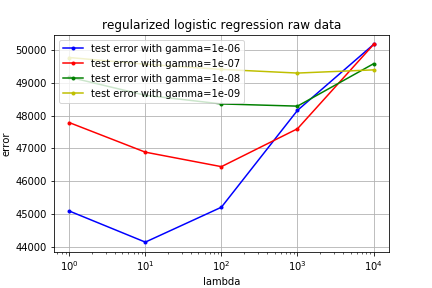
\includegraphics[width=\linewidth]{plots/raw_data_reg_log_regr.png}
  \caption{Regularized logistic regression - HP optimization}
  \label{fig:raw_reg_log_regr}
\end{figure}
\end{document}
